%\documentclass[notes,10pt,aspectratio=169]{beamer}

\documentclass[10pt,aspectratio=169]{beamer}

%\usetheme{Singapore} %Boadilla, Madrid, default, etc. 
\usetheme[progressbar=frametitle]{metropolis}
\usecolortheme{rose} %beaver, dolphin, crane, 




\usecolortheme{default}

\usepackage[utf8]{inputenc}
\usepackage[T1]{fontenc}
\usepackage{lmodern}
\usepackage{xcolor}
\usepackage{tikz}
\usetikzlibrary{shapes.geometric, arrows, positioning}

\tikzstyle{block} = [rectangle, draw, text width=4cm, align=center, rounded corners, minimum height=1cm]
\tikzstyle{decision} = [rectangle, draw, text width=5cm, align=center, fill=blue!10, rounded corners, minimum height=1cm]
\tikzstyle{terminal} = [rectangle, draw, text width=4.5cm, align=center, fill=yellow!30, rounded corners, minimum height=1cm]
\tikzstyle{end} = [rectangle, draw, text width=5cm, align=center, fill=green!30, rounded corners, minimum height=1cm]
\tikzstyle{arrow} = [->, thick]




%2. change the bullets 
\setbeamertemplate{itemize item}[triangle] %circle, square,... 


% 1. Define custom colors and set colors 
%\definecolor{myblue}{HTML}{003366}
\definecolor{accent}{RGB}{78,205,196}

%\setbeamercolor{title}{fg=white,bg=myblue}
\setbeamercolor{frametitle}{fg=black,bg=white}
%\setbeamercolor{normal text}{fg=mygray}
\setbeamercolor{block title}{fg=black,bg=blue}
%\setbeamercolor{block body}{fg=black,bg=white}

\setbeamercolor{item}{fg= orange!80} % Change bullet color
\setbeamercolor{button}{bg=orange, fg=white}





% 3. BibLaTeX settings
\usepackage[
  backend=biber,
  style=apa,
  citestyle=authoryear
]{biblatex}
\addbibresource{references.bib}

\title{Annuities system}
%\subtitle{A Mini Literature Overview}

\author{%
 Lucas Condeza
\inst{1} \and
   %\and
%  Coauthor Three\inst{3}
}
\institute{
  \inst{1} Yale University \\
%  \inst{2} University of X \\
%  \inst{3} University of Y
}

\date{\today}

\begin{document}

\begin{frame}
  \titlepage
\end{frame}



% Table of contents
%\begin{frame}{Outline}
%    \tableofcontents
%\end{frame}

% Section and slides

%\section{Introduction}

 

%%%%%%%%%%%%%%%%%%%%%%%
 


%%%%%%%%%%%%%%%%%%%%%%%%%

\begin{frame}{Institutional context} 
    \begin{itemize}%[<+->]
        \item Retirees choose between an annuity (Life Insurers, 60\% cases)   and \textit{phased withdrawals} (AFP)
        \begin{itemize}
            \item Annuities insure against risk due to long-life 
        \end{itemize}

    \item SCOMP system, steps: % how the annuities market works. 
    \begin{enumerate}
        \item Request of balance certificate to AFP % p. 51 in Quiroz et al 18 
        \item Request for offers: asks for certain type of contracts (e.g. annuity)
        \item Insurers make offers (e.g. \$1000 per month)
        \item Retiree chooses one of the offers or asks for external offers
    \end{enumerate}
        
    \item There are concerns about the lack of competition in the annuities market (FNE), caused by: 
        \begin{itemize}
            \item \textit{Unreasonable} choices. 25\% of the affiliates rejected offer 3.4\% higher than the one accepted (\cite{quiroz_estudio_2018})
            \item Intermediaries/brokers paid by insurance companies (\textcite{boehm_intermediation_nodate})
            
        \end{itemize}

    %\item Insurance companies see previous offers

    %\item Annuities  
\end{itemize} 
\end{frame}


%\begin{frame}{Frame Title}
%    \begin{figure}
%        \centering
%        \includegraphics[width=0.9\linewidth]{image.png}
%        \caption{Enter Caption}
%        \label{fig:enter-label}
%    \end{figure}
%\end{frame}



\begin{frame}{High rate heterogeneity}
\begin{figure}
    \centering
    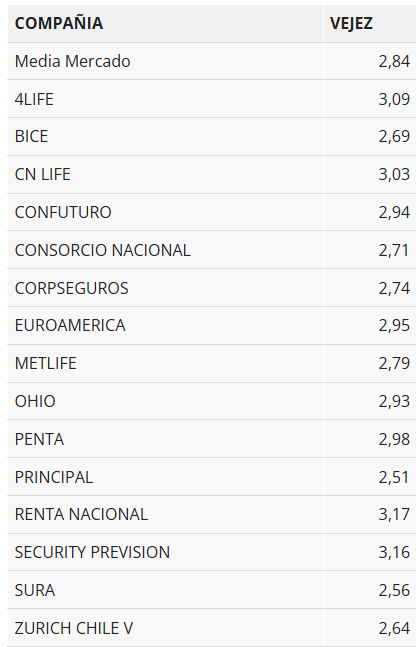
\includegraphics[width=0.5\linewidth]{../figures/image2.png}
    %\caption{Enter Caption}
    \label{fig:enter-label}
\end{figure}

 
\end{frame}



%\begin{frame}{Frame Title}
%\scalebox{0.65}{
%\begin{tikzpicture}[node distance=1cm and 1cm]

%% Top headings
%\node (aff) [block, fill=blue!10] {Affiliate};
%\node (part) [block, fill=blue!10, right=of aff] {Participant};
%\node (sys) [block, fill=blue!10, right=of part] {System};
%\node (prov) [block, fill=blue!10, right=of sys] {Providers};

%% First column
%\node (aff1) [block, below=1.2cm of aff] {1. Request certificate from AFP};
%\node (aff2) [block, below=0.7cm of aff1] {2. Choose participant: \\
%a) AFP (entering sales agent) \\
%b) Collective Severance (entering sales channel)};
%%\node (end1) [end, below=0.7cm of aff2, xshift=0.2cm] {c) Pensioning ends the pension process};

%% Second column
%\node (part3) [block, below=1.2cm of part] {3. Establish the offer request};
%\node (part4) [block, below=0.7cm of part3] {4. Send the request};
%\node (decision1) [decision, below=0.7cm of part4] { Affiliate chooses among: \\ a) accept internal offer, b) request external offer, c) new offer request};

%% Third column
%\node (sys5) [block, below=1.2cm of sys] {5. Validate the request};
%\node (sys6) [block, below=0.7cm of sys5] {6. System forwards offer request to AFPs and CSV};
%\node (sys8) [block, below=0.7cm of sys6] {8. System sends offers to affiliates};

%% Fourth column
%\node (prov7) [block, below=1.2cm of prov] {7. Providers send offers to system};

%% Output options
%%\node (respc) [decision, below=1.8cm of sys8, xshift=0cm] {c) Issue final offer response};
%%\node (nod) [terminal, below=0.6cm of respc] {d) Not pensioning};
%%\node (nod2) [terminal, below=1cm of decision1] {d) Not pensioning};

%% Arrows between blocks
%\draw[arrow] (aff) -- (aff1);
%\draw[arrow] (aff1) -- (aff2);
%%\draw[arrow] (aff2) -- (end1); %
%\draw[arrow] (aff2.east) -- ++(0.3,0) |- (part4.west);

%\draw[arrow] (part) -- (part3);
%\draw[arrow] (part3) -- (part4);
%\draw[arrow] (sys8) -- (decision1);

%%\draw[arrow] (decision1) -- ++(0,-1.2) -| (end1);
%%\draw[arrow] (decision1) -- (nod2);

%\draw[arrow] (sys) -- (sys5);
%\draw[arrow] (sys5) -- (sys6);
%%\draw[arrow] (prov7) -- (sys8);
%%\draw[arrow] (sys8) -- (respc);
%%\draw[arrow] (respc) -- (nod);

%\draw[arrow] (prov) -- (prov7);
%\draw[arrow] (prov7) -- ++(-0.3,-1) -- (sys8);

%%\draw[arrow] (respc.west) -- ++(-2,0) |- (decision1.east);

%\end{tikzpicture}
%}
%\end{frame}



%%%%%%%%%%%%%%%%%%%
%%%%%%%%%%%%%%%%%%%
%%%%%%%%%%%%%%%%%%%

 

%%%%%%%%%%%%%%%%%%%%%

\begin{frame}{Research questions}
\begin{itemize}
    %\item Whatare the impacts of being able to see previous offers? 
    \item Motivated by considerable policy interest
    \begin{itemize}
        \item What is the impact of allowing external offers? % The effect is ambiguous       
    \end{itemize}
    \item Why do affiliates reject better offers and potential solutions
        \begin{itemize}
            \item Highest offer as default option
        \end{itemize}
    %\item What role does interest risk play? 
\end{itemize}
\end{frame}


 \begin{frame}{Data}
\begin{itemize}
    \item SCOMP data at the individual level  
    \begin{itemize}
        \item Offers received and accepted 
        \item Total savings 
        \item Demographics: age, gender, etc. 
    \end{itemize}
     \item Retirement insurance companies: risk ratings, \#  of intermediaries and their  locations.
\end{itemize}
\end{frame}
 

\end{document}